
\section{Tosty francuskie na słono}
\bigskip
\small
\begin{minipage}{0.45\textwidth}
    \noindent \textbf{Czas:} 20 minut \\
    \textbf{Poziom trudności:} umiarkowany
\end{minipage}
\begin{minipage}{0.45\textwidth}
    \noindent \textbf{Ilość sprzątania:} średnia\\
    \textbf{Wymagany mysi sprzęt:} -
\end{minipage}
\normalsize
\vspace{0.5cm}

\begin{multicols}{2}

\subsection*{Składniki}
\begin{itemize}
    \item 2 jajka z wolnego wybiegu
    \item 0.5 szklanki mleka
    \item 2 dojrzałe pomidory lub odpowiadająca ilość pomidorków koktajlowych
    \item 4 kromki (najlepiej czerstwego) chleba lub chleba tostowego
    \item oliwa do smażenia
    \item przyprawy
    \item sól i pieprz do smaku
\end{itemize}

\columnbreak

\begin{figure}[H]
    \centering
    \fbox{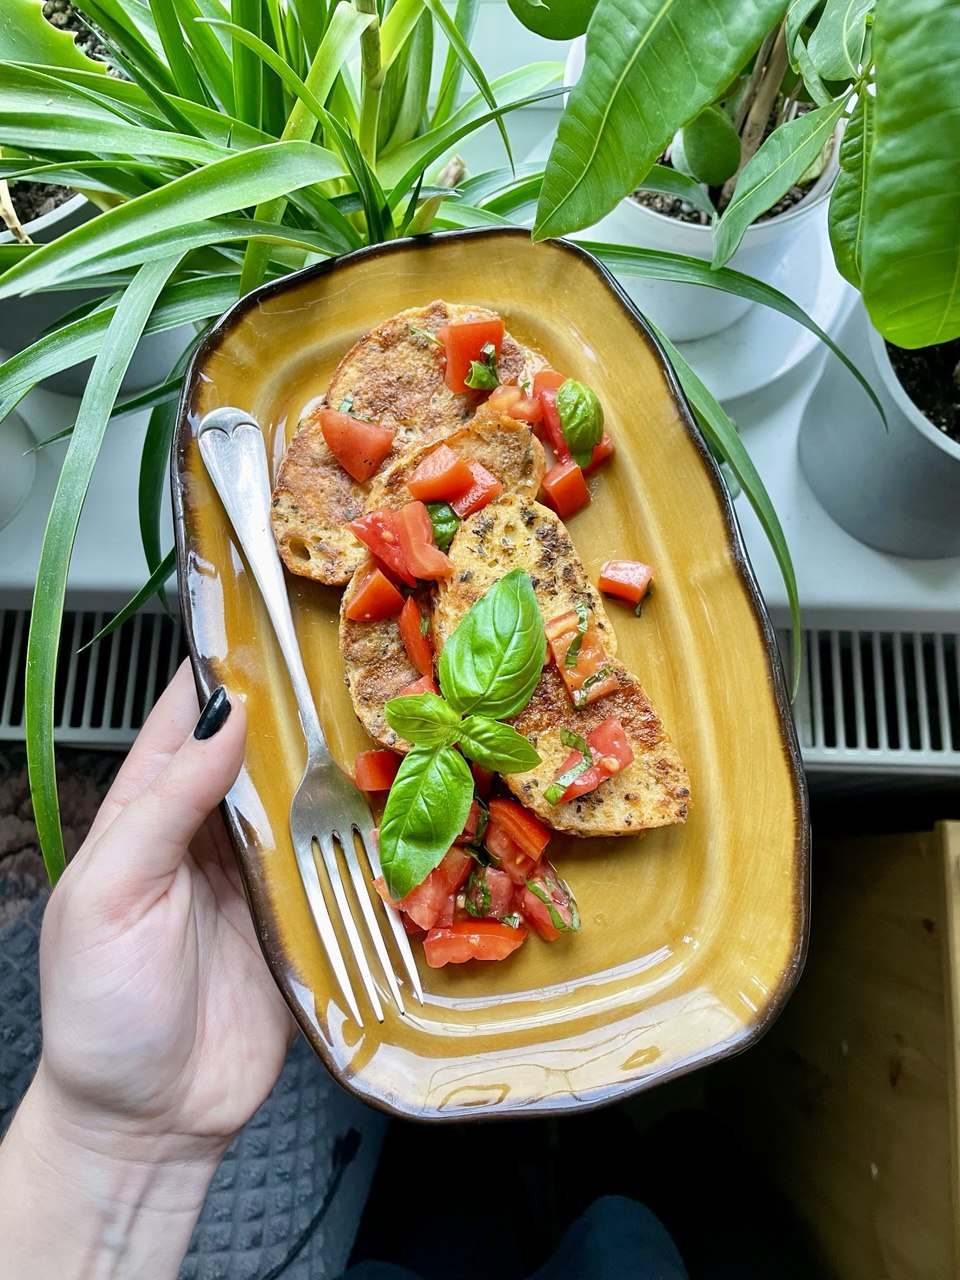
\includegraphics[width=0.35\textwidth]{images/tosty-na-slono.jpg}}
\end{figure}

\end{multicols}

\vspace{0.5cm}

\subsection*{Instruktaż}
\begin{enumerate}
    \item Pomidory pokroić w niewielką kostkę i przełożyć do miski. Doprawić odrobiną oliwy, płaską łyżeczką soli, pieprzu, majeranku, oregano, bazylii, tymianku, czosnku granulowanego. Wszystko dokładnie wymieszać i odstawić.
    \item Jajka roztrzepać z mlekiem i dodać po płaskiej łyżeczce soli, pieprzu i papryki słodkiej.
    \item Na rozgrzaną na średnim ogniu patelnię wlać oliwę i zaczekać, aż osiągnie temperaturę patelni. Kromki chleba pojedynczo lub parami namoczyć (ale nie rozmoczyć) w mieszance jajecznej z obu stron i smażyć na patelni z każdej strony, do momentu aż jajko się zetnie a tosty się zarumienią.
    \item Usmażone tosty przełożyć na talerz i serwować z krojonymi pomidorami.
\end{enumerate}

\vspace{0.5cm}

\small
\subsection*{Propozycja podania}
Z tartym serem, z listkami świeżej bazylii.

\vspace{0.3cm}

\subsection*{Dodatkowe uwagi}
Łatwo zamienić wytrawną wersję tostów na wersję na słodko - wystarczy mieszankę przypraw w miksturze jajecznej zastąpić niewielką ilością cukru i cynamonu, a zamiast z pomidorami serwować z dodatkami takimi jak jogurt, cukier puder, świeże owoce lub miód.

\newpage